% This is fft3d.tex, -*-LaTeX-*- 
% This document describes some crude models for the parallel
% decomposition of the Blue Matter application

%% 
%% ******************** IBM INTERNAL USE ONLY ************************* 
%% Copyright (C) 1994,1995 IBM Corporation 
%% 
%% This file is part of the IBM specific collection of LaTeX files 
%% for use internal to IBM. 
%% 
%% You are not allowed to distribute this file outside of IBM under 
%% any circumstances. 
%% 
%% If you have any questions, contact J. Hafner, hafner@almaden.ibm.com 
%% ******************************************************************** 
%%
%% These files are adapted from the old rj.sty files for use in
%% the new LaTeX2e.  There are many enhancements and a few bugs
%% have been fixed.  Undoubtedly there are many more.  Contact
%% the author if you find any or have suggestions for improvement
%% of this suite of files.
%% ********************************************************************
\NeedsTeXFormat{LaTeX2e}
\ProvidesFile{fft3d.tex}
           [1996/03/04 v1.2
   IBM ARC Research Report Sample]
%% \CharacterTable
%%  {Upper-case    \A\B\C\D\E\F\G\H\I\J\K\L\M\N\O\P\Q\R\S\T\U\V\W\X\Y\Z
%%   Lower-case    \a\b\c\d\e\f\g\h\i\j\k\l\m\n\o\p\q\r\s\t\u\v\w\x\y\z
%%   Digits        \0\1\2\3\4\5\6\7\8\9
%%   Exclamation   \!     Double quote  \"     Hash (number) \#
%%   Dollar        \$     Percent       \%     Ampersand     \&
%%   Acute accent  \'     Left paren    \(     Right paren   \)
%%   Asterisk      \*     Plus          \+     Comma         \,
%%   Minus         \-     Point         \.     Solidus       \/
%%   Colon         \:     Semicolon     \;     Less than     \<
%%   Equals        \=     Greater than  \>     Question mark \?
%%   Commercial at \@     Left bracket  \[     Backslash     \\
%%   Right bracket \]     Circumflex    \^     Underscore    \_
%%   Grave accent  \`     Left brace    \{     Vertical bar  \|
%%   Right brace   \}     Tilde         \~}
%%
%%
%\documentclass[dvips,finalversion,simpleeqnnos]{rjps}[1995/11/15]
\documentclass[pdftex,confidential,finalversion,simpleeqnnos]{rjps}[1995/11/15]
\pdfinfo{
  /Title (Distributed Transpose for Scalable Evaluation of Multi-dimensional FFTs on Massively Parallel Machines)
%/Author (Robert S. Germain)
}

\usepackage[LY1]{fontenc}       % specify text font encoding
\usepackage[expert]{lucidabr}
%\usepackage[mtbold]{mathtime}
\usepackage{amsmath}
\usepackage{graphicx}
\usepackage{rcsinfo}
% causes draft and revision number to printed across front page and
% at bottom of successive pages
%\usepackage[light, first, bottomafter]{draftcopy}
\usepackage{pdfdraftcopy}
%\usepackage{rcs}
%\usepackage{times}
\usepackage{hyperref}
\rcsInfo $Id: fft3d.tex 6256 2004-02-27 16:28:26Z rgermain $
%\RCS $Revision: 6256 $
\draftstring{DRAFT \rcsInfoRevision}
 % In the above, replace 'finalversion' by 'workingversion'
 % to get your labels and citations printed for easy cross referencing.
 % Using 'preliminaryversion' or none of these will print a draft
 % complete with cross references, but no cover page.
 %
 % Declare the title, author (use \email too!) and date.
 % Declare the title, author (use \email too!) and date.
\DeclareGraphicsExtensions{.pdf,.mps,.jpg,.png}
\bibliographystyle{plain}
\title{Distributed Transpose for Scalable Evaluation of Multi-dimensional FFTs on Massively Parallel Machines}
\author{R.S. Germain \and 
  B.G. Fitch \and
  Maria Eleftheriou \and
  A. Rayshubskiy \and
  T.J.C. Ward
\\[.5\baselineskip]  % give a little extra space to
  IBM Research Division\\       % set off the author names better 
  IBM Thomas J. Watson Research Center\\
  1101 Kitchawan Rd
  Route 134
  Yorktown Heights, NY 10598
}
%\date{\today}      % this won't appear on the cover page
\date{\rcsInfoLongDate}      % this won't appear on the cover page

 % These are optional, but place this information on the top of the
 % cover page:
%\rjnumber{RC 20994(92980) September 30, 1997}
\rjsubject{Computer Science}
%\appearedin{SPIE '95}

 % Now we have a place for keywords
\keywords{Parallel Programming, Molecular Dynamics,Fast Fourier Transform}

 % use this space for user-defined macros and environments
\newtheorem{theorem}{Theorem}

\newcommand{\Z}{\ensuremath{\mathbf{Z}}}
\newcommand{\R}{\ensuremath{\mathbf{R}}}
\newcommand{\udfcount}{\ensuremath{N^{udf}_{i}}}
\newcommand{\udftime}{\ensuremath{\tau^{udf}_{i}}}
\newcommand{\verlettime}{\ensuremath{\tau_{verlet}}}
\newcommand{\sitecount}{\ensuremath{{N_{sites}}}}
\newcommand{\rcutoff}{\ensuremath{r_{c}}}
\newcommand{\density}{\ensuremath{\rho}}
\newcommand{\nonbondtime}{\ensuremath{\tau_{non-bond}}}
\newcommand{\nodecount}{\ensuremath{P}}
\newcommand{\allreducetime}{\ensuremath{\tau_{AllReduce}(\sitecount,\nodecount)}}
\newcommand{\globalizepostime}{\ensuremath{\tau_{Globalize}(\sitecount, \nodecount)}}
\newcommand{\meshsize}[1]{\ensuremath{N_{#1}}}
\newcommand{\nodemeshsize}[1]{\ensuremath{\nodecount_{#1}}}
\newcommand{\nodecoord}[1]{\ensuremath{p_{#1}}}
\newcommand{\meshpernode}[1]{\ensuremath{n_{#1}}}
%\newcommand{\nodecoord}[1]{\ensuremath{c_{#1}}}
\newcommand{\pmetime}{\ensuremath{\tau_{p3me}(\nodecount,\meshsize)}}
\newcommand{\offset}[2]{\ensuremath{\Delta_{#1#2}}}

\begin{document}
\graphicspath{{./figures/},{../presentations/figures/}}
\pdfcatalog{
 /PageMode /UseOutlines
 }

\maketitle
%
% Here is the abstract which appears on the title page.
%
% Uncomment newpage to force the abstract on a new page. May especially
% be wanted in the report style.
%\newpage
\begin{abstract}
  This paper describes an implementation of a distributed transpose
  that enables scalability of a three-dimensional FFT beyond that
  obtainable with typical ``slab'' decomposition approaches. This
  implementation starts with a volumetric decomposition of the data
  across the 3-dimensional processor mesh.  It relies on the high
  performance torus interconnect and on strided accesses through local
  memory to carry out the distributed transposes efficiently and it
  can use any single-threaded one-dimensional FFT implementation as a
  building block.
\end{abstract}

\section{Introduction}

Three-dimensional Fast Fourier Transforms
(FFTs)\cite{zapata:1990,cramer:2000,ding:1995} are critical to a
number of numerical algorithms, in particular for the group of methods
termed ``Particle-Mesh'' or ``Particle-Particle-Particle-Mesh'' which
are used in N-body simulations of systems with electrostatic
forces.\cite{hockney:1988}

This paper describes an implementation of a distributed
three-dimensional FFT that allows scalability beyond that obtainable
with typical ``slab'' decomposition approaches. This implementation
starts with a volumetric decomposition of the data across the
3-dimensional processor mesh.  To evaluate an $N\times N\times N$ FFT,
it uses the ``row-column'' method to decompose the problem into
successive evaluations of $N^2$ one-dimensional FFTs along each axis.
Without parallelizing the evaluation of the individual 1-d FFTs, the
concurrency inherent in the computational phase for this method allows
scaling to $N^2$ nodes.  It relies on the high performance torus
interconnect, an efficient distribution scheme across processors, and
on strided accesses through local memory to carry out the distributed
transposes efficiently.  Although it was developed for mesh/torus
architectures, it also works efficiently on other high performance
network topologies.

\subsection{Multi-dimensional FFT}
% The definitions are shamelessly copied from Jorg Arndt's Algorithms
% for Programmers document at http://www.jjj.de/fxt/
Consider the d-dimensional array $a_{\bf x}$ of dimensions $N_0\times
N_1\times N_2\times\ldots\times N_{d-1}$ where ${\bf x} =
(x_0,x_1,x_2,\ldots,x_{d-1}), x_i \in \Z_{N_{i}}$.  The Fourier
transform $\hat{a}_{\bf k} = \mathcal{F}_{\bf x}^d[a]$ consisting of a d-dimensional array of
$N_0\,N_1\,N_2\,\ldots\,N_{d-1}$ numbers where  ${\bf k} =
(k_0,k_1,k_2,\ldots,k_{d-1}), k_i \in \Z_{N_{i}}$ is defined by:
\begin{eqnarray}
\hat{a}_{\bf k} & = &
\frac{1}{\sqrt{n}}\,\sum_{x_0=0}^{N_0-1}\,\sum_{x_1=0}^{N_1-1}\,\cdots\,\sum_{x_{d-1}=0}^{N_{d-1}}a_{\bf
  x}\,\prod_{l=0}^{d-1}\exp(2\pi\imath\,x_l\,k_l/N_l) \\
          & = &
\frac{1}{\sqrt{N_0}}\,\sum_{x_0=0}^{N_0-1}\exp(2\pi\imath\,x_0\,k_0/N_0)\,
\frac{1}{\sqrt{N_1}}\,\sum_{x_1=0}^{N_1-1}\exp(2\pi\imath\,x_1\,k_1/N_1)\,
\cdots\,\nonumber \\
& & \mbox{} \frac{1}{\sqrt{N_{d-1}}}\,\sum_{x_{d-1}=0}^{N_{d-1}}\exp(2\pi\imath\,x_{d-1}\,k_{d-1}/N_{d-1})a_{\bf
  x} \nonumber \\
& = & \mathcal{F}_{x_0}^{1}\circ\mathcal{F}_{x_1}^{1}\circ\cdots
\circ\mathcal{F}_{x_{d-1}}^{1}[a] \nonumber
\end{eqnarray}

For the target scientific application, system sizes are such that mesh
dimensions of 64$^3$ or 128$^3$ are most common.  For small node count
systems, a ``slab'' decomposition of the FFT onto an array of
processors is most efficient.  However, this would only allow mapping
of the FFT onto partitions with at most 64 or 128 nodes.  In
principle, there is plenty of work to distribute over a much larger
number of nodes since there are $3\times\meshsize{}^2$ 1D FFTs to be
computed overall.  Assuming that the 1D FFT is not to be parallelized,
each stage in the 3D FFT requires $\meshsize{}^2$ 1D FFT computations.
Figure~\ref{fig:fft_dflow} shows the dataflows for FFT-related computations
required to solve Poisson's equation for the P3ME method.

Since BG/L is a torus/mesh machine, it is natural to use a volume
decomposition to map the 3D mesh domain onto the machine.  Assuming
that the domain mesh dimensions are $\meshsize{0}\times
\meshsize{1}\times \meshsize{2}$ and that the machine partition size is
$\nodecount=\nodemeshsize{0}\times \nodemeshsize{1}\times \nodemeshsize{2}$ then each node will have responsibility
for $(\meshsize{0}/\nodemeshsize{0})\times (\meshsize{1}/\nodemeshsize{1})\times (\meshsize{2}/\nodemeshsize{2})$ mesh points. During
each phase of the naive decomposition of the 3D FFT illustrated in
Figure~\ref{fig:fft_dflow}, communication occurs along rows of nodes
in a particular direction.  The process looks like this:
\begin{enumerate}
\item Each node in the row sends $\nodemeshsize{i}-1$ messages to the other nodes
  in the row.  Each message contains $(\meshsize{0}/\nodemeshsize{0})\times (\meshsize{1}/\nodemeshsize{1})\times
  (\meshsize{2}/\nodemeshsize{2})\times (1/\nodemeshsize{i})\times \mbox{sizeof}(\mbox{complex})$ bytes.
\item Each node carries out $(\meshsize{j}/\nodemeshsize{j})\times (\meshsize{k}/\nodemeshsize{k})\times (1/\nodemeshsize{i})$
  one-dimensional FFTs on local data.
\item Each node in the row sends $\nodemeshsize{i}-1$ messages to the other nodes
  in the row.  Each message contains $(\meshsize{0}/\nodemeshsize{0})\times (\meshsize{1}/\nodemeshsize{1})\times
  (\meshsize{2}/\nodemeshsize{2})\times (1/\nodemeshsize{i})\times \mbox{sizeof}(\mbox{complex})$ bytes.
\end{enumerate}

For example, a 512 node partition (8$\times$8$\times$8) working on a
128$\times$128$\times$128 mesh implies a total data volume leaving or
entering each node of:
\begin{displaymath}
2\times 8\times 7\times \frac{128}{8}\times \frac{128}{8}\times
\frac{128}{8}\times \frac{1}{8}\times \mbox{sizeof}(\mbox{double})
\end{displaymath}

\begin{figure}
\begin{center}
\includegraphics[keepaspectratio,width=0.9\textwidth]{fft0.mps}
\end{center}
\caption{Schematic view of dataflow and candidate partitioning keys
  for the computations of the convolution required for the P3ME method.}
\label{fig:fft_dflow}
\end{figure}

\begin{figure}
\begin{center}
\includegraphics[keepaspectratio,width=0.5\textwidth]{fft1.mps}
\end{center}
\caption{Schematic view of the data partitioning within a column and
  the message paths required.}
\label{fig:fft_column}
\end{figure}

\begin{figure}
\begin{center}
\includegraphics[keepaspectratio,width=0.8\textwidth]{fft2.mps}
\end{center}
\caption{Schematic view of the data partitioning within a column and
  the message paths required.}
\label{fig:fft_column2}
\end{figure}
\section{Multi-dimensional FFT of a Real Function}

For the case where $a_{\mathbf{x}}$ is real, the transformed data have
additional symmetries that can be used to save computations and/or
space.  For convenience, we will write:
\begin{eqnarray}
\hat{a}(k_0, k_1,\ldots,k_l,x_{l+1},x_{l+2},\ldots,x_{d-1} &=&\nonumber \\
\hat{a}(\mathbf{\hat{k}},\mathbf{\hat{x}}) &=&\nonumber \\
&=& \mathcal{F}_{x_0}^{1}\circ\mathcal{F}_{x_1}^{1}\circ\cdots\circ\mathcal{F}_{x_l}^{1}[a] \nonumber
\end{eqnarray}
If $a_{\mathbf{x}} \in \R$ then $a_{\mathbf{x}}^{*} = a_{\mathbf{x}}$
which implies that:
\begin{displaymath}
\hat{a}(\mathbf{\hat{k}},\mathbf{\hat{x}})^{*} =
\hat{a}(-\mathbf{\hat{k}},\mathbf{\hat{x}}) \nonumber
\end{displaymath}

\section{Routing/Distribution of Data in Complex 3D-FFT}

The sequence of distribution and operations for the forward part of a
3D-FFT intended for use in convolution looks like this:
\begin{equation}
\begin{array}{ccccccc}
  & & FFT(z) & & FFT(y) & & FFT(x) \\
  (x, y, z)& \longrightarrow & (x, y) & \longrightarrow & (x, k_z) &
  \longrightarrow & (k_y, k_z)
\end{array}
\end{equation}

\subsection{Phase I: Transform along the Z-direction}

At the beginning of the first phase, the mesh points are distributed
in a volume decomposition on the processor mesh so that
$\meshsize{x}\times\meshsize{y}\times\meshsize{z}$ mesh points are
distributed over $\nodemeshsize{x}\times\nodemeshsize{y}\times\nodemeshsize{z}$
processors. Each processor will contain
$(\meshsize{x}/\nodemeshsize{x})\times
(\meshsize{y}/\nodemeshsize{y})\times (\meshsize{z}/\nodemeshsize{z})
= \meshpernode{x}\times\meshpernode{y}\times\meshpernode{z}$
mesh points, where $\meshpernode{i} \equiv
\meshsize{i}/\nodemeshsize{i}$.  For convenience, we will define the
relative coordinate
of a mesh point within a processor as
\begin{eqnarray}
\delta x & \equiv & x - \lfloor x/\meshpernode{x}
\rfloor\,\meshpernode{x} \\
\delta y & \equiv & y - \lfloor y/\meshpernode{y}
\rfloor\,\meshpernode{y} \\
\delta z & \equiv & z - \lfloor z/\meshpernode{z}
\rfloor\,\meshpernode{z}
\end{eqnarray}
and the processor coordinate $(\nodecoord{x}, \nodecoord{y},
\nodecoord{z})$ for mesh coordinate $(x, y, z)$ is
\begin{equation}
(\nodecoord{x}, \nodecoord{y}, \nodecoord{z}) = (\lfloor
  x/\meshpernode{x} \rfloor, \lfloor y/\meshpernode{y} \rfloor, \lfloor
  z/\meshpernode{z} \rfloor)
\end{equation}
where the floor function $\lfloor x \rfloor$ is the greatest integer
less than or equal to $x$, $x \in \Z_{\meshsize{x}}$, $y \in
\Z_{\meshsize{y}}$, and $z \in \Z_{\meshsize{z}}$.

During this first phase, all of the meshpoints corresponding to a
particular pair of $x$ and $y$ coordinates must be mapped the same
processor so that the one-dimensional FFT can be performed along the
z-coordinate.  One mapping of $(x, y)$ to the processor requires only
communications along the z-direction so that
% ME: modify the p_Z^dest
\begin{eqnarray}
\nodecoord{x}^{dest} & = & \left\lfloor \frac{x}{\meshpernode{x}} \right\rfloor \\
\nodecoord{y}^{dest} & = & \left\lfloor \frac{y}{\meshpernode{y}} \right\rfloor \\
\nodecoord{z}^{dest} & = & \left\lfloor \frac{ ( \delta y +
  \meshpernode{y}\,\delta x  ) \,\nodemeshsize{z} }{\meshpernode{x}\,\meshpernode{y}}\right\rfloor
\end{eqnarray}

This mapping attempts to keep ranges of $y$ values together because
the next phase involves one-dimensional FFTs along the y-coordinate.

We would also like to be able to calculate what range of $\delta x$
and $\delta y$ is sent to a particular node $\nodecoord{z}$.  Let us
define the offset

\begin{equation}
\offset{y}{x} \equiv \delta y + \meshpernode{y}\,\delta x \label{eqn:delta_def_xy}
\end{equation}
so that
%ME: modify the delta_{x}
\begin{eqnarray}
\delta x & = & \left\lfloor
\frac{\offset{y}{x}}{\meshpernode{y}} \right\rfloor \label{eqn:def_delta_x} \\
\delta y & = & \offset{y}{x} \bmod \meshpernode{y} \label{eqn:def_delta_y}
\end{eqnarray}
and
%ME: modify the p_z^dest
\begin{displaymath}
\nodecoord{z}^{dest} = \left\lfloor
\frac{\offset{y}{x}\,\nodemeshsize{z} }{\meshpernode{x}\,\meshpernode{y}}\right\rfloor.
\end{displaymath}
%ME: modify the p_z^dest
Given this expression for $\nodecoord{z}^{dest}$, we can say that
\begin{displaymath}
\nodecoord{z}^{dest} \leq
\frac{\offset{y}{x}\,\nodemeshsize{z}}{\meshpernode{x}\,\meshpernode{y}}
\end{displaymath}
and
%ME: modify the p_z^dest
\begin{displaymath}
\nodecoord{z}^{dest} + 1 >
\frac{\offset{y}{x}\,\nodemeshsize{z}}{\meshpernode{x}\,\meshpernode{y}}
\end{displaymath}
implying that
%ME: modify the upper limit
\begin{equation}
\frac{\meshpernode{x}\,\meshpernode{y}\,\nodecoord{z}^{dest}}{\nodemeshsize{z}}
\leq \offset{y}{x} <
\frac{\meshpernode{x}\,\meshpernode{y}\,(\nodecoord{z}^{dest} +
1)}{\nodemeshsize{z}} 
\end{equation}
One can write the expression for the range of $\offset{y}{x}$ in the following
form:
%ME: Modify upper limit
\begin{equation}
\offset{y}{x} \in \left [ 
  \frac{\meshpernode{x}\,\meshpernode{y} \, \nodecoord{z}^{dest}}{\nodemeshsize{z}},
\frac{\meshpernode{x}\,\meshpernode{y}\,(\nodecoord{z}^{dest} +
1)}{\nodemeshsize{z}}
\right )\label{eqn:delta_range_xy}
\end{equation}
%\offset{y}{x} \in \left [ \left\lfloor
%  \frac{\meshpernode{x}\,\meshpernode{y}}{\nodemeshsize{z}}\,\nodecoord{z}^{dest}
%  \right\rfloor, \left\lfloor
%  \frac{\meshpernode{x}\,\meshpernode{y}}{\nodemeshsize{z}}\,\nodecoord{z}^{dest}
%  + \frac{\meshpernode{x}\,\meshpernode{y}}{\nodemeshsize{z}}
%  \right\rfloor \right ) \label{eqn:delta_range_xy}.


The actual $x$ and $y$ offsets can be calculated from $\offset{y}{x}$
using the expressions:
\begin{eqnarray}
\delta x &=& \left\lfloor \frac{\offset{y}{x}}{\meshpernode{y}}
\right\rfloor \\
\delta y &=& \offset{y}{x} \bmod \meshpernode{y}
\end{eqnarray}

\subsection{Phase II: Transform along the Y-direction}

At the beginning of this phase, the values corresponding to the full
range of z values have been transformed into values corresponding to a
range of k$_z$ values. If we were trying to be ``neat'', we might want
to transform the distribution of mesh points so that the data defined
over the mesh $(x, y, k_z)$ were distributed in a volume decomposition
over the processor mesh so that $(\nodecoord{x}, \nodecoord{y},
\nodecoord{z}) = (\lfloor x/\nodemeshsize{x} \rfloor, \lfloor
y/\nodemeshsize{y} \rfloor, \lfloor k_z/\nodemeshsize{z} \rfloor)$.
However, we need to then map all mesh points with same $x$ and $k_z$
values to the same node so that the one-dimensional FFTs along the
y-coordinate can be performed.  An example of a mapping appropriate
for this end that involves communication along the $y$ and $z$
processor axes is
%\begin{eqnarray}
%\nodecoord{x}^{dest} & = & \left\lfloor \frac{x}{\meshpernode{x}} \right\rfloor \\
%\nodecoord{y}^{dest} & = & \left\lfloor\frac{\delta x +
%  \meshpernode{x}\,(k_z-\meshpernode{z}\,\lfloor
%  k_z/\meshpernode{z}\rfloor)}{\meshpernode{x}\,\meshpernode{z}}\,\nodemeshsize{y} \right\rfloor \\
%& = & \left\lfloor\frac{\delta x + \meshpernode{x}\,\delta
 % k_z}{\meshpernode{x}\,\meshpernode{z}}\,\nodemeshsize{y}
%\right\rfloor \nonumber \\ 
%\nodecoord{z}^{dest} & = & \left\lfloor\frac{k_z}{\meshpernode{z}}\right\rfloor
%\end{eqnarray}

\begin{eqnarray}
\nodecoord{x}^{dest} & = & \left\lfloor \frac{x}{\meshpernode{x}} \right\rfloor \\
\nodecoord{y}^{dest} & = & \left\lfloor\frac{\delta x +
  \meshpernode{x}\,(k_z-\meshpernode{z}\,\lfloor
  k_z/\meshpernode{z}\rfloor)\,\nodemeshsize{y}}{\meshpernode{x}\,\meshpernode{z}} \right\rfloor \\
& = & \left\lfloor\frac{(\delta x + \meshpernode{x}\,\delta
 k_z )\,\nodemeshsize{y}}{\meshpernode{x}\,\meshpernode{z}}
\right\rfloor \nonumber \\ 
\nodecoord{z}^{dest} & = & \left\lfloor\frac{k_z}{\meshpernode{z}}\right\rfloor
\end{eqnarray}


where $\delta k_z \equiv k_z-\meshpernode{z}\,\lfloor
k_z/\meshpernode{z}\rfloor$.

This mapping attempts to keep ranges of $x$ values together because
the next and final phase involves one-dimensional FFTs along the
x-coordinate.

We can define $\offset{x}{k_z} \equiv \delta x + \meshpernode{x}\delta
k_z$ and write down an expression for the range of $\offset{x}{k_z}$
analogous to Equation~\ref{eqn:delta_range_xy}:
\begin{equation}
\offset{x}{k_z} \in \left [ \left\lceil
  \frac{\meshpernode{x}\,\meshpernode{z} \,\nodecoord{y}^{dest}}{\nodemeshsize{y}}
  \right\rceil, \left\lceil
  \frac{\meshpernode{x}\,\meshpernode{z}\,\nodecoord{y}^{dest}}{\nodemeshsize{y}}
  + \frac{\meshpernode{x}\,\meshpernode{z}}{\nodemeshsize{y}}
  \right\rceil \right ) \label{eqn:delta_range_xkz}
\end{equation}

\subsection{Phase III: Transform along the X-direction}

At the beginning of this phase our mesh points are distributed over
$(x, k_y, k_z)$ and the mapping to processors has all mesh points
corresponding to particular values of $x$ and $k_z$ mapped to the same
processor. By analogy with the expressions for Phase II and in order
to keep ranges of $k_y$ values together because of the order of
transforms required for the inverse 3D-FFT to follow, we write an
expression for a possible mapping to processors


\begin{eqnarray}
\nodecoord{x}^{dest} & = & \left\lfloor\frac{(\delta k_y + \meshpernode{y}\,\delta
  k_z ) \,\nodemeshsize{x} }{\meshpernode{y}\,\meshpernode{z}}
\right\rfloor \\ 
\nodecoord{y}^{dest} & = &
\left\lfloor\frac{k_y}{\meshpernode{y}}\right\rfloor \\
\nodecoord{z}^{dest} & = & \left\lfloor\frac{k_z}{\meshpernode{z}}\right\rfloor
\end{eqnarray}
where $\delta k_y \equiv k_y-\meshpernode{y}\,\lfloor
k_y/\meshpernode{y}\rfloor$.

\section{Preliminary Results}

Many of the results reported thus far use a preliminary implementation
of the addressing scheme that does not give full scalability of the
work outlined here. The very first piece of work reported used a 512
node Power4 system as a test platform and the results of that work and
a comparison with FFTW\cite{FFTW98} are shown in
Figure~\ref{fig:fftw_compare}.  Figure~\ref{fig:fft3d_meas} shows the
performance achieved thus far using a variety of one-dimensional FFT
building blocks including FFTW's uniprocessor FFT as well as a
home-brewed version adapted from Reference~\cite{press:93}.
\begin{figure}
\includegraphics[keepaspectratio,
width=\textwidth]{fftbench_128_compare.mps}
\caption{Comparison of a preliminary version of the volumetric FFT
  with the 3D-FFTW (\url{http://www.fftw.org}) library on a 512
  processor Power4 cluster.  Note that while FFTW's ``slab''
  decomposition flattens out at high node counts, the volumetric FFT
  continues to increase in speed through 512 nodes.}
\label{fig:fftw_compare}
\end{figure}

\begin{figure}
\includegraphics[keepaspectratio,
width=\textwidth]{fftbg_compare_speedups.mps}
\caption{Measured speedups of a preliminary version of the volumetric
  FFT on both Power4 and BG/L prototype hardware.}
\label{fig:fft3d_speedups}
\end{figure}

\begin{figure}
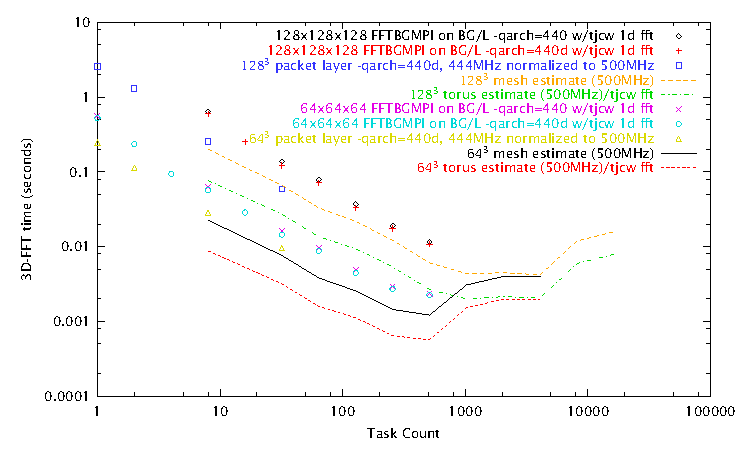
\includegraphics[keepaspectratio,
width=\textwidth]{fftbgmpi_with_estimate_20031116.mps}
  \caption{Measured execution times of preliminary versions of the volumetric 3D-FFT on both Power4 and BG/L prototype hardware.  Comparisons with models using designed hardware capabilities are shown as well.}
  \label{fig:fft3d_meas}
\end{figure}

%\bibliography{/u/germain/tex/bibliography/vision,/u/germain/tex/bibliography/software}
\bibliography{../bibliography/fft,../bibliography/md,../bibliography/fftw}

\end{document}
